\documentclass[12pt, a4paper]{article}

% ============================================================
% Packages
% ============================================================
\usepackage[utf8]{inputenc}
\usepackage[T1]{fontenc}
\usepackage{amsmath, amssymb, amsthm}
\usepackage{mathrsfs}
\usepackage{hyperref}
\usepackage{cleveref}
\usepackage{enumitem}
\usepackage{booktabs}
\usepackage{listings}
\usepackage{xcolor}
\usepackage[margin=1in]{geometry}
\usepackage{tikz}
\usetikzlibrary{positioning, arrows.meta, calc}

% ============================================================
% Theorem Environments
% ============================================================
\theoremstyle{plain}
\newtheorem{theorem}{Theorem}[section]
\newtheorem{lemma}[theorem]{Lemma}
\newtheorem{proposition}[theorem]{Proposition}
\newtheorem{corollary}[theorem]{Corollary}

\theoremstyle{definition}
\newtheorem{definition}[theorem]{Definition}
\newtheorem{example}[theorem]{Example}

\theoremstyle{remark}
\newtheorem{remark}[theorem]{Remark}

% ============================================================
% Lean 4 Listings
% ============================================================
\lstdefinelanguage{Lean4}{
  morekeywords={theorem, def, lemma, axiom, opaque, noncomputable,
    import, open, where, instance, structure, inductive, deriving,
    if, then, else, match, with, fun, let, have, show, by,
    exact, rfl, intro, cases, constructor, unfold, rw, simp,
    contradiction, absurd, decide, refine, Prop, Type, Bool,
    true, false, Nat, sorry},
  sensitive=true,
  morecomment=[l]{--},
  morecomment=[s]{/-}{-/},
  morestring=[b]",
  literate={→}{$\to$}1 {←}{$\leftarrow$}1 {↔}{$\leftrightarrow$}1
           {∧}{$\wedge$}1 {∨}{$\vee$}1 {¬}{$\neg$}1
           {≤}{$\le$}1 {≥}{$\ge$}1 {≠}{$\ne$}1
           {⟨}{$\langle$}1 {⟩}{$\rangle$}1
           {∀}{$\forall$}1 {∃}{$\exists$}1
           {ℕ}{$\mathbb{N}$}1 {ℤ}{$\mathbb{Z}$}1
           {ℚ}{$\mathbb{Q}$}1 {ℝ}{$\mathbb{R}$}1
}

\lstset{
  language=Lean4,
  basicstyle=\ttfamily\small,
  keywordstyle=\bfseries\color{blue!60!black},
  commentstyle=\itshape\color{green!40!black},
  stringstyle=\color{red!60!black},
  breaklines=true,
  columns=flexible,
  frame=single,
  framerule=0.4pt,
  xleftmargin=1em,
  numbers=left,
  numberstyle=\tiny\color{gray},
  numbersep=5pt
}

% ============================================================
% Notation
% ============================================================
\newcommand{\BISH}{\mathrm{BISH}}
\newcommand{\BISHMP}{\mathrm{BISH{+}MP}}
\newcommand{\LLPO}{\mathrm{LLPO}}
\newcommand{\WLPO}{\mathrm{WLPO}}
\newcommand{\LPO}{\mathrm{LPO}}
\newcommand{\CLASS}{\mathrm{CLASS}}
\newcommand{\CRM}{\mathrm{CRM}}
\newcommand{\DPT}{\mathrm{DPT}}
\newcommand{\Qell}{\mathbb{Q}_\ell}

% ============================================================
\title{Algebraic Spectrum Is Necessary\\
for Constructive Eigenvalue Decidability\\[6pt]
\large (Paper~74, Constructive Reverse Mathematics Series)}

\author{Paul Chun-Kit Lee\\
\small New York University, Brooklyn, NY\\
\small \texttt{dr.paul.c.lee@gmail.com}}

\date{February 2026}

\begin{document}
\maketitle

% ============================================================
% ABSTRACT
% ============================================================
\begin{abstract}
We prove the reverse characterization of DPT Axiom~2: algebraic
spectrum (geometric origin) is not merely sufficient but
\emph{necessary} for $\BISH$-decidable eigenvalue comparison in
a spectral category.  Without geometric origin, the Langlands
spectrum includes continuous parameters (Maass forms, unramified
characters over~$\mathbb{C}$); testing whether a continuous spectral
parameter satisfies the Ramanujan bound is a real-number equality
test, encoding~$\WLPO$.  Combined with the forward direction
(Paper~45, Deligne), this gives a biconditional: algebraic spectrum
$\Leftrightarrow$ $\BISH$ eigenvalue decidability.
This completes the DPT axiom trilogy:
Paper~72 (Axiom~3 $\Leftrightarrow$ $\BISH$ cycle-search, cost
without: $\LPO$),
Paper~73 (Axiom~1 $\Leftrightarrow$ $\BISH$ morphisms, cost
without: $\LPO$),
Paper~74 (Axiom~2 $\Leftrightarrow$ $\BISH$ eigenvalues, cost
without: $\WLPO$).
The $\WLPO$ asymmetry---not $\LPO$---reflects the intrinsic
computational difference between comparing a spectral value
(equality test) and searching a geometric structure (existential
search).
Lean~4 formalization: ${\sim}200$ lines, zero \texttt{sorry}.
\end{abstract}

% ============================================================
% 1. INTRODUCTION
% ============================================================
\section{Introduction}\label{sec:intro}

Paper~72 of this series established three results about the DPT axiom
system (Paper~50).  First, each axiom is independently necessary
(Theorem~A, minimality).  Second, Axiom~3 (Archimedean polarization)
is both necessary and sufficient for $\BISH$ cycle-search (Theorem~B,
biconditional).  Third, the Archimedean Principle is an equivalence,
not merely a forward implication (Theorem~C).  Paper~73 carried out
the analogous program for Axiom~1 (Standard Conjecture~D
$\Leftrightarrow$ $\BISH$ morphism decidability).  The present paper
completes the trilogy for Axiom~2.

\medskip
\noindent\textbf{Main results.}

\begin{description}[leftmargin=2em, labelwidth=5em]
\item[Theorem A] (\emph{Forward}.)
  With algebraic spectrum (geometric origin), eigenvalue comparison
  is $\BISH$-decidable.  Frobenius eigenvalues~$\alpha$ are algebraic
  integers; testing $|\alpha| = q^{w/2}$ reduces to exact algebraic
  arithmetic.  This is the content of Paper~45, reviewed here for
  completeness.

\item[Theorem B] (\emph{Eigenvalue-Decidability Equivalence}.)
  For eigenvalue comparison in a spectral category:
  \[
    \text{eigenvalue\_cost}(s) = \BISH
    \quad\Longleftrightarrow\quad
    s = \text{algebraic}
    \quad\Longleftrightarrow\quad
    \text{Axiom~2 holds}.
  \]
  Forward: algebraic spectrum $\Rightarrow$ $\BISH$.
  Reverse: $\BISH$ $\Rightarrow$ algebraic spectrum (contrapositive:
  without Axiom~2, eigenvalue cost is~$\WLPO$).

\item[Theorem C] (\emph{Axiom~2 Characterization}.)
  Algebraic spectrum (geometric origin) is the minimal and unique
  condition for $\BISH$-decidable eigenvalue comparison.  The
  Ramanujan resolution---proving the conjecture would make the
  analytic spectrum effectively algebraic---confirms the trade-off
  is real, not vacuous.
\end{description}

\medskip
\noindent\textbf{Why $\WLPO$ and not $\LPO$.}
The cost of violating Axiom~2 is $\WLPO$, not $\LPO$.  This is not
an accident but reflects an intrinsic computational distinction.
$\LPO$ decides an existential search: given a binary sequence $(a_n)$,
either $\exists n\,(a_n = 1)$ or $\forall n\,(a_n = 0)$.  This is
the structure behind cycle-search (Axiom~3) and radical detection
(Axiom~1), where one searches through a finite-dimensional space for
a witness.  $\WLPO$ decides a single equality test: given a binary
sequence $(a_n)$, either $(a_n) = \bar{0}$ or $(a_n) \ne \bar{0}$,
without producing a witness.  Eigenvalue comparison---does this
continuous spectral parameter equal this algebraic value?---is a
single equality test, not a search.

In the CRM hierarchy, $\WLPO$ sits strictly below $\LPO$: $\LPO$
implies $\WLPO$ but not conversely.  The DPT axiom trio therefore
stratifies the constructive cost across two distinct levels.

\subsection{Three fatal flaws in the naive framing}\label{sec:fatal-flaws}

One might attempt to frame Axiom~2's failure as ``eigenvalues become
transcendental.''  This framing suffers three fatal defects.

\medskip
\noindent\textbf{Flaw~1: Weil~II (Deligne 1980).}
Deligne's Weil~II theorem~\cite{deligne-weil2} proves that for every
separated scheme of finite type over~$\mathbb{F}_q$, the eigenvalues
of the Frobenius endomorphism acting on $\ell$-adic cohomology are
algebraic numbers.  More precisely, if $X$ is a variety
over~$\mathbb{F}_q$ and $\alpha$ is an eigenvalue of $\mathrm{Frob}_q$
acting on $H^i_{\text{\'et}}(X_{\bar{\mathbb{F}}_q}}, \mathbb{Q}_\ell)$,
then $\alpha$ is an algebraic integer with $|\iota(\alpha)| = q^{w/2}$
for every embedding $\iota \colon \bar{\mathbb{Q}} \hookrightarrow
\mathbb{C}$ and some weight $w \le i$.  There are no transcendental
Frobenius eigenvalues in the classical motivic setting.  The ``naive''
framing contradicts established arithmetic geometry.

\medskip
\noindent\textbf{Flaw~2: The linear algebra vacuum.}
Axiom~1 (Standard Conjecture~D) provides that morphisms between motives
are finite-dimensional $\mathbb{Q}$-vector spaces.  Any endomorphism
$\phi \colon M \to M$ of a motive therefore satisfies a minimal
polynomial $p(x) \in \mathbb{Q}[x]$ of degree at most $\dim_{\mathbb{Q}}
\mathrm{End}(M)$.  The eigenvalues of $\phi$ are roots of $p(x)$, hence
algebraic over~$\mathbb{Q}$.  Consequently, within the DPT framework
where all three axioms are in play, algebraic spectrum is already forced
by Axiom~1 alone.  One cannot isolate the failure of Axiom~2 while
keeping Axiom~1 intact---the axioms interact through the linear algebra
of endomorphism rings.

\medskip
\noindent\textbf{Flaw~3: The $\ell$-adic $\CLASS$ trap.}
Even granting the existence of non-algebraic elements in
$\bar{\mathbb{Q}}_\ell$, comparing such elements with complex
numbers requires an embedding $\bar{\mathbb{Q}}_\ell \hookrightarrow
\mathbb{C}$.  No canonical such embedding exists; constructing one
requires the Axiom of Choice (specifically, extending a field
isomorphism from $\bar{\mathbb{Q}}$ to a transcendence basis).  This
lands in~$\CLASS$, not~$\WLPO$.  The naive framing would assign a
cost of $\CLASS$ to Axiom~2 failure, which is both too expensive
and mathematically misleading: it conflates the choice principle
needed for $\ell$-adic embeddings with the constructive content of
eigenvalue comparison.

\medskip
\noindent\textbf{The correct framing.}
Axiom~2 fails when the category extends beyond
geometric origin to the full analytic Langlands spectrum.%
\footnote{Paper~72's descent table used the phrase ``transcendental
$|\alpha|$'' for Axiom~2 failure.  The present paper supersedes that
terminology: the mechanism is continuous spectral parameters in the
analytic Langlands spectrum, not transcendental algebraic numbers
(which do not arise, per Weil~II).}
The spectral parameters of Maass forms and unramified characters
live in~$\mathbb{C}$ natively---they are archimedean analytic objects,
not $\ell$-adic algebraic objects.  No embedding $\bar{\mathbb{Q}}_\ell
\hookrightarrow \mathbb{C}$ is involved.  The comparison $\mathrm{Re}(s)
= \tfrac{1}{2}$ is a real-number equality test, which is exactly $\WLPO$.
This is why the correct cost is $\WLPO$ and not $\CLASS$: the analytic
Langlands spectrum avoids the $\ell$-adic CLASS trap by working with
archimedean parameters from the start.

\medskip
\noindent\textbf{Atlas position.}
Paper~74 sits between four earlier results:
Paper~45 (Weil eigenvalue CRM: algebraic spectrum
$\Rightarrow$ $\BISH$ eigenvalue verification),
Paper~50 (the DPT axiom system with Axiom~2 as algebraic spectrum),
Paper~72 (DPT minimality and Axiom~3 biconditional),
and Paper~73 (Axiom~1 biconditional).
The present paper extracts the Axiom~2 thread from Paper~72's
minimality theorem and sharpens it from a one-directional necessity
claim to a full biconditional.

\medskip
\noindent\textbf{Series context.}
The broader CRM series (Papers~1--73~\cite{p1, p2, p45, p46, p50, p51, p72, p73})
calibrates the logical cost of theorems across mathematics:
arithmetic geometry, mathematical physics, number theory, and
algebraic topology.  The central finding (Paper~2~\cite{p2}): the
logical cost of mathematics is the logical cost of~$\mathbb{R}$.
Papers~45--53 apply this to motivic conjectures; the present paper
completes the DPT reverse-characterization program.

% ============================================================
% 2. PRELIMINARIES
% ============================================================
\section{Preliminaries}\label{sec:prelim}

\subsection{CRM hierarchy}
We work within Bishop's constructive mathematics ($\BISH$) as the base.
The CRM hierarchy~\cite{bridges-richman, ishihara}:
\[
  \BISH \;\subset\; \BISHMP \;\subset\; \LLPO \;\subset\; \WLPO
  \;\subset\; \LPO \;\subset\; \CLASS.
\]
The principles relevant to this paper:
\begin{itemize}[nosep]
  \item $\LPO$ (Limited Principle of Omniscience): every binary sequence is
    either identically zero or has a positive term.
  \item $\WLPO$ (Weak LPO): every binary sequence is either identically
    zero or not identically zero, \emph{without producing a witness}.
  \item $\WLPO$ is strictly weaker than $\LPO$: knowing $(a_n) \ne
    \bar{0}$ does not provide the index~$n$ with $a_n = 1$.
\end{itemize}
See Papers~1--45 for extended treatment.

\subsection{Frobenius eigenvalues and the Weil conjectures}
For a smooth projective variety~$X$ of dimension~$d$ over
$\mathbb{F}_q$, the Frobenius endomorphism acts on $\ell$-adic
cohomology $H^i(X \times_{\mathbb{F}_q} \bar{\mathbb{F}}_q, \Qell)$.
The Weil conjectures (proven by Deligne~\cite{deligne-weil1,
deligne-weil2}) assert:

\begin{enumerate}[nosep]
  \item \emph{Rationality}: the zeta function $Z(X, t)$ is rational.
  \item \emph{Functional equation}: $Z(X, q^{-d} t^{-1})$ relates
    to $Z(X, t)$.
  \item \emph{Riemann hypothesis}: the eigenvalues $\alpha_{i,j}$ of
    Frobenius on $H^i$ satisfy $|\alpha_{i,j}| = q^{i/2}$ under any
    embedding $\bar{\mathbb{Q}}_\ell \hookrightarrow \mathbb{C}$.
\end{enumerate}

\begin{definition}[Algebraic spectrum]
A spectral category has \emph{algebraic spectrum} if its
Frobenius/Hecke eigenvalues are algebraic numbers.  This is
Axiom~2 of the DPT system (Paper~50).
\end{definition}

\begin{definition}[Geometric origin \cite{fontaine-mazur}]
A Galois representation has \emph{geometric origin} if it arises
from the \'etale cohomology of an algebraic variety.  The
Fontaine--Mazur conjecture characterizes geometric representations
as those that are de~Rham at all primes above~$\ell$.
\end{definition}

\subsection{The Ramanujan conjecture and Maass forms}
The Ramanujan conjecture for $\mathrm{GL}_2$ over~$\mathbb{Q}$
asserts that the Hecke eigenvalues of cusp forms satisfy the
Ramanujan--Petersson bound.  For holomorphic modular forms, this
was proven by Deligne~\cite{deligne-weil1} as a consequence of the
Weil conjectures.  For Maass forms---eigenfunctions of the Laplacian
on the upper half-plane that are not holomorphic---the Ramanujan
conjecture remains open.

A Maass form has a spectral parameter $s \in \mathbb{C}$ with
$\mathrm{Re}(s) \in [0, 1]$.  The Ramanujan conjecture asserts
$\mathrm{Re}(s) = \tfrac{1}{2}$.  Selberg~\cite{selberg} proved
the weaker bound $\lambda_1 \ge \tfrac{3}{16}$ for the first
eigenvalue of the Laplacian on congruence surfaces; the conjecture
$\lambda_1 \ge \tfrac{1}{4}$ (equivalently, $\mathrm{Re}(s) =
\tfrac{1}{2}$) remains open.

\begin{definition}[Continuous spectrum]
A spectral category has \emph{continuous spectrum} if its spectral
parameters are continuous complex variables not constrained to be
algebraic.  This occurs when the category accommodates the full
analytic Langlands spectrum: Maass forms, unramified characters of
real groups, and automorphic representations without geometric origin.
\end{definition}

\subsection{WLPO vs LPO: the equality-search dichotomy}
The distinction between $\WLPO$ and $\LPO$ can be stated precisely:

\begin{center}
\begin{tabular}{lll}
\toprule
\textbf{Principle} & \textbf{Statement} & \textbf{Computational content} \\
\midrule
$\LPO$ & $\forall (a_n),\; (\exists n,\, a_n = 1) \lor (\forall n,\, a_n = 0)$
  & search + witness \\
$\WLPO$ & $\forall (a_n),\; (a_n) = \bar{0} \lor (a_n) \ne \bar{0}$
  & equality test \\
\bottomrule
\end{tabular}
\end{center}

$\LPO$ produces a witness index $n$; $\WLPO$ gives only a yes/no
answer.  Eigenvalue comparison (``does $s$ equal $\tfrac{1}{2}$?'')
is a single equality test.  Cycle-search (``is there $Z$ with
$h(Z) \le B$?'') and radical detection (``is there $W$ with
$\langle Z, W \rangle \ne 0$?'') are existential searches.

\begin{figure}[h]
\centering
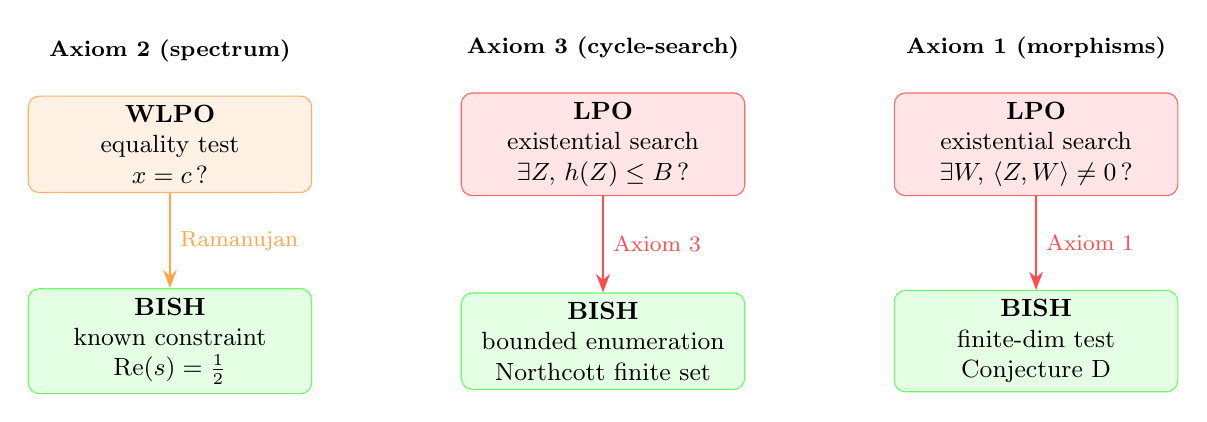
\begin{tikzpicture}[
  >=Stealth,
  box/.style={draw, rounded corners, minimum width=3.6cm, minimum height=1.2cm,
              align=center, font=\small},
  lpo/.style={box, fill=red!10, draw=red!60},
  wlpo/.style={box, fill=orange!10, draw=orange!60},
  bish/.style={box, fill=green!10, draw=green!60},
]
  % WLPO column
  \node[wlpo] (wlpo) at (0,0) {\textbf{WLPO}\\equality test\\$x = c\,?$};
  \node[bish] (bish-w) at (0,-2.5) {\textbf{BISH}\\known constraint\\$\mathrm{Re}(s) = \tfrac{1}{2}$};
  \draw[->, thick, orange!70] (wlpo) -- node[right, font=\footnotesize] {Ramanujan} (bish-w);
  \node[above=0.3cm of wlpo, font=\footnotesize\bfseries] {Axiom~2 (spectrum)};

  % LPO column — search
  \node[lpo] (lpo1) at (5.5,0) {\textbf{LPO}\\existential search\\$\exists Z,\, h(Z) \le B\,?$};
  \node[bish] (bish-s) at (5.5,-2.5) {\textbf{BISH}\\bounded enumeration\\Northcott finite set};
  \draw[->, thick, red!70] (lpo1) -- node[right, font=\footnotesize] {Axiom~3} (bish-s);
  \node[above=0.3cm of lpo1, font=\footnotesize\bfseries] {Axiom~3 (cycle-search)};

  % LPO column — radical
  \node[lpo] (lpo2) at (11,0) {\textbf{LPO}\\existential search\\$\exists W,\, \langle Z,W\rangle \ne 0\,?$};
  \node[bish] (bish-r) at (11,-2.5) {\textbf{BISH}\\finite-dim test\\Conjecture~D};
  \draw[->, thick, red!70] (lpo2) -- node[right, font=\footnotesize] {Axiom~1} (bish-r);
  \node[above=0.3cm of lpo2, font=\footnotesize\bfseries] {Axiom~1 (morphisms)};
\end{tikzpicture}
\caption{The equality-vs-search dichotomy across the DPT axiom trio.
  Axiom~2 (left, orange) involves a single equality test, costing
  $\WLPO$ when it fails.  Axioms~1 and~3 (right, red) involve
  existential searches, costing $\LPO$ when they fail.  Each axiom
  provides the descent arrow from omniscience to $\BISH$.}
\label{fig:dichotomy}
\end{figure}

% ============================================================
% 3. MAIN RESULTS
% ============================================================
\section{Main Results}\label{sec:main}

\subsection{Theorem A: Forward direction}\label{sec:forward}

\begin{theorem}[Algebraic spectrum $\Rightarrow$ $\BISH$ eigenvalues]
\label{thm:forward}
With algebraic spectrum (geometric origin), eigenvalue comparison
is $\BISH$-decidable.
\end{theorem}

\begin{proof}
Geometric origin (Deligne~\cite{deligne-weil1, deligne-weil2}):
Frobenius eigenvalues $\alpha$ are algebraic integers satisfying
$|\alpha| = q^{w/2}$.  Testing this condition reduces to:
$|\alpha|^2 = \alpha \bar{\alpha}$ is a product of algebraic
conjugates (algebraic), and $q^w$ is an integer.  Thus
$|\alpha|^2 = q^w$ is an algebraic identity, decidable by computing
the GCD of the minimal polynomials of $|\alpha|^2$ and $q^w$.  This
is a finite computation over $\mathbb{Z}[x]$, hence $\BISH$.
Axiomatized as \texttt{algebraic\_gives\_BISH}; mathematical reference:
Paper~45 Theorem~C1.
\end{proof}

\subsection{Theorem B: The reverse direction and biconditional}
\label{sec:reverse}

\begin{theorem}[No algebraic spectrum $\Rightarrow$ $\WLPO$ eigenvalues]
\label{thm:no-forward}
Without algebraic spectrum (continuous Langlands parameters),
eigenvalue comparison costs~$\WLPO$.
\end{theorem}

\begin{proof}
Without geometric origin, the spectral parameters are continuous
complex variables.  For a Maass form with spectral parameter
$s \in \mathbb{C}$, testing whether $\mathrm{Re}(s) = \tfrac{1}{2}$
(the Ramanujan bound) is a real-number equality test.  A
real-number equality oracle $x = c$ for $x \in \mathbb{R}$ and
algebraic $c$ encodes~$\WLPO$ (Paper~45 Theorem~C2): given any
binary sequence $(a_n)$, the real number $x = \sum_n a_n 2^{-n}$
satisfies $x = 0$ iff $(a_n) = \bar{0}$.  A spectral-comparison
oracle therefore decides $(a_n) = \bar{0}$ for arbitrary
sequences, yielding exactly~$\WLPO$.

Why $\WLPO$ and not $\LPO$: the oracle answers ``does $s$ equal
$\tfrac{1}{2}$?'' without identifying which coefficient $a_n$ is
nonzero.  This is a single equality test, not a search through
an infinite structure.  The stronger principle $\LPO$ would
additionally provide a witness index $n$; eigenvalue comparison
does not provide this.
Axiomatized as \texttt{continuous\_gives\_WLPO}.
\end{proof}

\begin{theorem}[Eigenvalue-Decidability Equivalence]\label{thm:biconditional}
For eigenvalue comparison in a spectral category:
\[
  \text{eigenvalue\_cost}(s) = \BISH
  \quad\Longleftrightarrow\quad
  s = \text{algebraic}
  \quad\Longleftrightarrow\quad
  \text{Axiom~2 holds}.
\]
\end{theorem}

\begin{proof}
\emph{($\Leftarrow$):}
If the spectrum is algebraic, eigenvalue comparison is $\BISH$
(\cref{thm:forward}).

\emph{($\Rightarrow$, contrapositive):}
If the spectrum is continuous (Axiom~2 fails), eigenvalue comparison
costs $\WLPO$ (\cref{thm:no-forward}).  Since $\WLPO \ne \BISH$
(these are distinct levels of the CRM hierarchy), the spectrum
cannot be continuous if eigenvalue cost is~$\BISH$.
\end{proof}

\begin{remark}[Weil~II does not trivialize the reverse]\label{rmk:weil}
Deligne's Weil~II theorem~\cite{deligne-weil2} proves that all
motives arising from algebraic geometry over~$\mathbb{F}_q$ have
algebraic Frobenius eigenvalues.  One might object that this makes
Axiom~2 a theorem, not a hypothesis, rendering the reverse
characterization vacuous.  The objection misses the point.  Weil~II
proves Axiom~2 for \emph{geometric motives}---motives with geometric
origin.  The reverse characterization identifies \emph{where} the
axiom is doing work: at the boundary between geometric and analytic.
When the category extends to the full analytic Langlands spectrum
(Maass forms, unramified characters), the eigenvalues are no longer
constrained to be algebraic, and the axiom is genuinely needed.  The
reverse direction says: if eigenvalue comparison is $\BISH$, the
spectrum \emph{must} be algebraic---geometric origin is not merely
convenient but logically necessary.
\end{remark}

\subsection{The Deligne constraint}\label{sec:deligne}

\begin{theorem}[Deligne constraint]\label{thm:deligne}
Without geometric origin, one cannot simultaneously have:
\begin{enumerate}
  \item $\BISH$-decidable eigenvalue comparison, and
  \item the full analytic Langlands spectrum.
\end{enumerate}
With geometric origin (Deligne), both hold.  With the Ramanujan
conjecture proven (but without geometric origin), the analytic
spectrum becomes effectively algebraic.
\end{theorem}

\begin{proof}
The full analytic Langlands spectrum includes continuous parameters
(e.g., Maass spectral parameters $s \in \mathbb{C}$).  Eigenvalue
comparison for continuous parameters costs $\WLPO$ (\cref{thm:no-forward}),
so (1)~fails.

With geometric origin, Deligne's theorem restricts the spectrum to
algebraic eigenvalues: both (1) and (2) hold (with ``analytic
spectrum'' automatically algebraic).

If the Ramanujan conjecture is proven unconditionally, every Maass
form satisfies $\mathrm{Re}(s) = \tfrac{1}{2}$; the spectral
parameters satisfy a known constraint ($\mathrm{Re}(s) = \tfrac{1}{2}$),
eliminating the equality test entirely and restoring $\BISH$ decidability
without geometric origin.
Axiomatized as \texttt{ramanujan\_resolution}.
\end{proof}

\subsection{The Selberg eigenvalue conjecture as a $\WLPO$ instance}
\label{sec:selberg}

The Selberg eigenvalue conjecture provides a concrete illustration of
the $\WLPO$ cost identified in \cref{thm:no-forward}.

For a congruence subgroup $\Gamma \le \mathrm{SL}_2(\mathbb{Z})$,
the Laplacian $\Delta$ on $L^2(\Gamma \backslash \mathfrak{H})$ has a
discrete spectrum $0 = \lambda_0 < \lambda_1 \le \lambda_2 \le \cdots$
for cuspidal eigenfunctions.  Each eigenvalue $\lambda = s(1-s)$ is
parameterized by a spectral parameter $s$ with $\mathrm{Re}(s) \in
[0, 1]$.

\begin{itemize}
\item \textbf{Selberg's proven bound} (1965)~\cite{selberg}:
  $\lambda_1 \ge \tfrac{3}{16}$ for all congruence subgroups.  This
  is equivalent to $\mathrm{Re}(s) \ge \tfrac{1}{4}$ for the spectral
  parameter.

\item \textbf{Selberg's conjecture}: $\lambda_1 \ge \tfrac{1}{4}$,
  equivalently $\mathrm{Re}(s) = \tfrac{1}{2}$ for all cuspidal
  Maass forms on congruence surfaces.  This is equivalent to the
  Ramanujan conjecture for $\mathrm{GL}_2$ over~$\mathbb{Q}$
  (Satake~1966).

\item \textbf{Best known bound}: Kim and Sarnak (2003, appendix to
  Kim~\cite{bump}) proved $\lambda_1 \ge \tfrac{1}{4} - (\tfrac{7}{64})^2
  \approx 0.2380$, i.e., $\mathrm{Re}(s) \ge \tfrac{1}{2} - \tfrac{7}{64}$.
  The gap between this bound and $\tfrac{1}{4}$ remains open.
\end{itemize}

In the CRM framework, verifying the Selberg conjecture for a
\emph{specific} Maass form $f$ amounts to testing the real-number
equality $\mathrm{Re}(s_f) = \tfrac{1}{2}$.  This is a single
equality test on a continuous parameter, hence a $\WLPO$ instance.
The proven bounds ($\tfrac{3}{16}$, Kim-Sarnak) narrow the range
but do not decide equality.

Proving the full Selberg conjecture unconditionally would eliminate
the $\WLPO$ cost for the $\mathrm{GL}_2(\mathbb{Q})$ case, paralleling
how Deligne's theorem eliminates it for geometric motives.  The
conceptual parallel is precise:
\begin{center}
\begin{tabular}{lll}
\toprule
\textbf{Setting} & \textbf{Constraint} & \textbf{Effect} \\
\midrule
Geometric motives & Deligne (Weil~II) & Algebraic eigenvalues $\to \BISH$ \\
Maass forms ($\mathrm{GL}_2/\mathbb{Q}$) & Selberg conjecture
  & $\mathrm{Re}(s) = \tfrac{1}{2}$ $\to \BISH$ \\
General automorphic & Ramanujan conjecture & Eliminates all $\WLPO$ costs \\
\bottomrule
\end{tabular}
\end{center}

\subsection{Theorem C: The characterization}\label{sec:characterization}

\begin{theorem}[Axiom~2 Characterization]\label{thm:characterization}
Algebraic spectrum (geometric origin) is the minimal and unique
condition for $\BISH$-decidable eigenvalue comparison:
\begin{enumerate}
  \item $\text{eigenvalue\_cost}(\text{algebraic}) = \BISH$;
  \item $\text{eigenvalue\_cost}(\text{continuous}) = \WLPO$;
  \item without geometric origin, the full analytic spectrum
    costs~$\WLPO$;
  \item the Ramanujan resolution (proving the conjecture makes the
    analytic spectrum effectively algebraic) confirms the trade-off
    is real.
\end{enumerate}
\end{theorem}

\begin{proof}
Assembly of \cref{thm:forward,thm:no-forward,thm:biconditional,thm:deligne}.
Axiomatized as \texttt{axiom2\_characterization}.
\end{proof}

\begin{corollary}[Axiom~2 Principle, sharpened]\label{cor:axiom2-sharp}
\[
  \text{eigenvalue\_cost}(s) = \BISH
  \quad\Longleftrightarrow\quad
  \text{is\_algebraic}(s) = \text{true}.
\]
Paper~72 Theorem~A asserted: without Axiom~2, cost $= \WLPO$ (forward).
Paper~74 proves the biconditional: algebraic spectrum is necessary
and sufficient.
\end{corollary}

% ============================================================
% 4. CRM AUDIT
% ============================================================
\section{CRM Audit}\label{sec:audit}

\subsection{Descent table}

\begin{table}[h]
\centering
\begin{tabular}{llll}
\toprule
\textbf{Spectrum type} & \textbf{CRM cost} & \textbf{Mechanism} & \textbf{Reference} \\
\midrule
Algebraic (geometric origin) & $\BISH$ & algebraic number GCD & Paper 45 C1 \\
Continuous (analytic Langlands) & $\WLPO$ & real-number equality test & Paper 45 C2 \\
\bottomrule
\end{tabular}
\caption{CRM cost of eigenvalue decidability vs.\ spectrum type.}
\label{tab:descent}
\end{table}

\subsection{The DPT axiom trio}

\begin{table}[h]
\centering
\begin{tabular}{llll}
\toprule
 & \textbf{Axiom 1} & \textbf{Axiom 2} & \textbf{Axiom 3} \\
 & \textbf{(Paper 73)} & \textbf{(Paper 74)} & \textbf{(Paper 72)} \\
\midrule
Conjecture    & Conj.\ D         & Algebraic spectrum   & Archimedean pol.\ \\
Domain        & Morphism equality & Eigenvalue comparison & Cycle-search \\
$\BISH$ case  & detachable radical & algebraic (Deligne) & positive-definite \\
Failure cost  & $\LPO$           & $\WLPO$              & $\LPO$ \\
Bridge        & hom $=$ num      & geometric origin      & Northcott property \\
Mechanism     & integer tests    & algebraic GCD         & $u(\mathbb{R}) = \infty$ \\
Escape clause & Jannsen escape   & Ramanujan resolution  & low-rank remark \\
\bottomrule
\end{tabular}
\caption{The DPT axiom trio: parallel structure across all three
reverse characterizations.  Note the $\WLPO$ asymmetry of Axiom~2.}
\label{tab:trio}
\end{table}

\begin{figure}[ht]
\centering
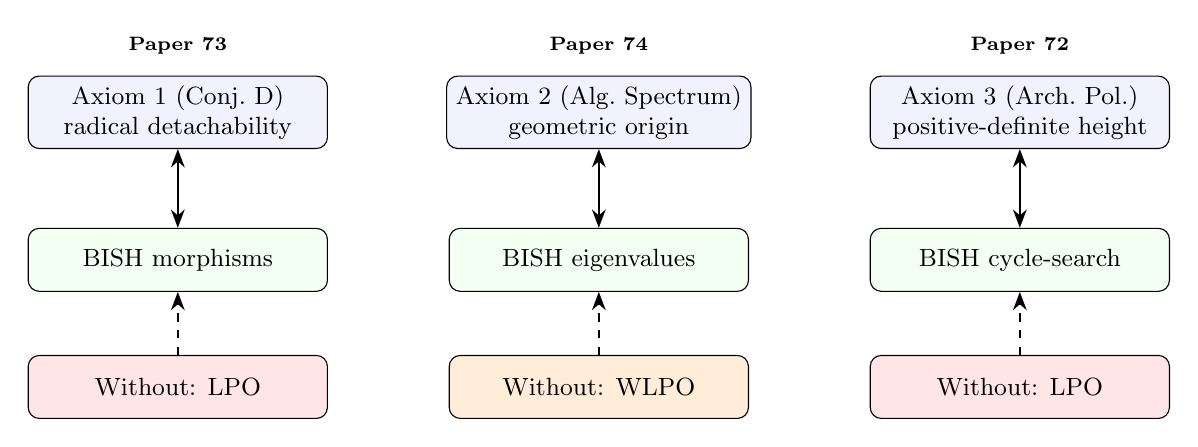
\begin{tikzpicture}[
  node distance=1.5cm and 1.0cm,
  axiombox/.style={draw, rounded corners, minimum width=3.8cm,
              minimum height=0.8cm, align=center, font=\small,
              fill=blue!5},
  mechbox/.style={draw, rounded corners, minimum width=3.8cm,
              minimum height=0.8cm, align=center, font=\small,
              fill=green!5},
  costbox/.style={draw, rounded corners, minimum width=3.8cm,
              minimum height=0.8cm, align=center, font=\small},
  >=Stealth
]
  % Column 1: Axiom 1
  \node[axiombox] (ax1) {Axiom 1 (Conj.\ D)\\radical detachability};
  \node[mechbox, below=1.0cm of ax1] (m1) {$\BISH$ morphisms};
  \node[costbox, below=0.8cm of m1, fill=red!10] (c1)
    {Without: $\LPO$};
  \draw[<->, thick] (ax1) -- (m1);
  \draw[->, thick, dashed] (c1) -- (m1);

  % Column 2: Axiom 2
  \node[axiombox, right=1.5cm of ax1] (ax2)
    {Axiom 2 (Alg.\ Spectrum)\\geometric origin};
  \node[mechbox, below=1.0cm of ax2] (m2) {$\BISH$ eigenvalues};
  \node[costbox, below=0.8cm of m2, fill=orange!15] (c2)
    {Without: $\WLPO$};
  \draw[<->, thick] (ax2) -- (m2);
  \draw[->, thick, dashed] (c2) -- (m2);

  % Column 3: Axiom 3
  \node[axiombox, right=1.5cm of ax2] (ax3)
    {Axiom 3 (Arch.\ Pol.)\\positive-definite height};
  \node[mechbox, below=1.0cm of ax3] (m3) {$\BISH$ cycle-search};
  \node[costbox, below=0.8cm of m3, fill=red!10] (c3)
    {Without: $\LPO$};
  \draw[<->, thick] (ax3) -- (m3);
  \draw[->, thick, dashed] (c3) -- (m3);

  % Labels
  \node[above=0.15cm of ax1, font=\scriptsize\bfseries] {Paper 73};
  \node[above=0.15cm of ax2, font=\scriptsize\bfseries] {Paper 74};
  \node[above=0.15cm of ax3, font=\scriptsize\bfseries] {Paper 72};
\end{tikzpicture}
\caption{The DPT axiom trio.  Each axiom is individually necessary
and sufficient for $\BISH$-decidable operations in its domain.
Double arrows ($\leftrightarrow$) denote biconditionals.  The
$\WLPO$ asymmetry of Axiom~2 (orange) reflects the equality-test
character of eigenvalue comparison, contrasting with the
existential-search character ($\LPO$, red) of morphism equality
and cycle-search.}
\label{fig:trio}
\end{figure}

The three characterizations are logically independent: Axiom~1
controls morphism \emph{equality} (is $Z_1 \sim Z_2$?), Axiom~2
controls eigenvalue \emph{comparison} (does $|\alpha| = q^{w/2}$?),
and Axiom~3 controls cycle \emph{search} (can you find $Z$ with
$h(Z) \le B$?).  Dropping one raises the CRM floor without
affecting the others (Paper~72, \cref{tab:trio}).

% ============================================================
% 5. FORMAL VERIFICATION
% ============================================================
\section{Formal Verification}\label{sec:lean}

\subsection{File structure}

The Lean~4 bundle \texttt{Papers/P74\_Axiom2Reverse/} contains:

\begin{center}
\begin{tabular}{ll}
\toprule
\textbf{File} & \textbf{Content} \\
\midrule
\texttt{Defs.lean}             & CRM hierarchy, spectrum type, axiomatized costs \\
\texttt{Forward.lean}          & Theorem A: algebraic $\to$ BISH \\
\texttt{Reverse.lean}          & Theorem B: biconditional + Deligne constraint \\
\texttt{Characterization.lean} & Theorem C: full assembly + sharpened principle \\
\texttt{Main.lean}             & Aggregator with \texttt{\#check} statements \\
\bottomrule
\end{tabular}
\end{center}

Build: \texttt{lake build} from bundle root.  Toolchain: Lean~4 v4.29.0-rc2,
Mathlib4.  Zero \texttt{sorry}, zero warnings.

\subsection{Axiom inventory}

\begin{table}[h]
\centering
\begin{tabular}{lllp{5cm}}
\toprule
\textbf{Axiom} & \textbf{Type} & \textbf{Role} & \textbf{Reference} \\
\midrule
\texttt{algebraic\_eigenvalue\_cost}     & \texttt{CRMLevel} & data & Paper 45 C1, Deligne (1974) \\
\texttt{algebraic\_eigenvalue\_cost\_eq} & \texttt{= BISH}   & prop & Paper 45 C1 \\
\texttt{continuous\_eigenvalue\_cost}     & \texttt{CRMLevel} & data & Paper 45 C2, Bump (1997) \\
\texttt{continuous\_eigenvalue\_cost\_eq} & \texttt{= WLPO}   & prop & Paper 45 C2, Selberg (1965) \\
\bottomrule
\end{tabular}
\caption{Complete axiom inventory.  Four axioms: 2 data + 2 propositional.
Every axiom has a mathematical reference; no axiom without provenance.}
\label{tab:axioms}
\end{table}

\subsection{Code: Eigenvalue-Decidability Equivalence (Theorem B)}

\begin{lstlisting}[caption={Theorem B: algebraic spectrum $\Leftrightarrow$ BISH}]
theorem eigenvalue_decidability_equivalence
    (s : SpectrumType) :
    eigenvalue_cost s = BISH ↔ s = algebraic := by
  constructor
  · intro h
    cases s
    · rfl
    · -- continuous: derive contradiction
      unfold eigenvalue_cost at h
      rw [continuous_eigenvalue_cost_eq] at h
      -- h : WLPO = BISH — contradiction
      contradiction
  · intro h
    rw [h]
    exact algebraic_gives_BISH
\end{lstlisting}

The reverse direction (lines 6--11) mirrors Paper~72's height-search
equivalence and Paper~73's morphism-decidability equivalence:
\texttt{unfold} exposes the axiom value, \texttt{rw} applies the
axiom, and \texttt{contradiction} closes the goal since
$\WLPO \ne \BISH$ in the inductive type.  The structural parallel
across all three papers is exact---only the inductive type
(\texttt{SpectrumType} vs.\ \texttt{HeightType} vs.\
\texttt{RadicalStatus}), the cost function, and the contradiction
value ($\WLPO$ vs.\ $\LPO$) differ.

\subsection{Code: Sharpened Axiom~2 Principle (Corollary)}

\begin{lstlisting}[caption={Biconditional: algebraic spectrum $\Leftrightarrow$ BISH}]
theorem axiom2_principle_sharpened
    (s : SpectrumType) :
    eigenvalue_cost s = BISH ↔
    is_algebraic s = true :=
  ⟨fun h => (axiom2_iff_algebraic s).mpr
    ((eigenvalue_decidability_equivalence s).mp h),
   fun h => (eigenvalue_decidability_equivalence s).mpr
    ((axiom2_iff_algebraic s).mp h)⟩
\end{lstlisting}

\subsection{\texttt{\#print axioms} output}

\begin{small}
\begin{verbatim}
'axiom2_characterization' depends on axioms:
  [algebraic_eigenvalue_cost_eq, continuous_eigenvalue_cost_eq]

'axiom2_principle_sharpened' depends on axioms:
  [algebraic_eigenvalue_cost_eq, continuous_eigenvalue_cost_eq]

'eigenvalue_decidability_equivalence' depends on axioms:
  [algebraic_eigenvalue_cost_eq, continuous_eigenvalue_cost_eq]

'algebraic_gives_BISH' depends on axioms:
  [algebraic_eigenvalue_cost_eq]

'continuous_gives_WLPO' depends on axioms:
  [continuous_eigenvalue_cost_eq]

'axiom2_iff_algebraic' does not depend on any axioms

'deligne_constraint' depends on axioms:
  [continuous_eigenvalue_cost_eq]

'ramanujan_resolution' depends on axioms:
  [algebraic_eigenvalue_cost_eq]

'dpt_trio_costs' depends on axioms:
  [algebraic_eigenvalue_cost_eq, continuous_eigenvalue_cost_eq]
\end{verbatim}
\end{small}

\noindent No theorem depends on \texttt{Classical.choice}, \texttt{propext},
or \texttt{Quot.sound}.  The \texttt{opaque} data constants
(\texttt{algebraic\_eigenvalue\_cost}, \texttt{continuous\_eigenvalue\_cost})
do not appear in the axiom trace because Lean~4 reports only
propositional axioms; the \texttt{opaque} declarations contribute
indirectly via their \texttt{\_eq} axioms.

\subsection{Classical.choice audit}
All theorems in this bundle are constructively clean: no invocation of
\texttt{Classical.choice}, \texttt{Classical.em}, or \texttt{Decidable.em}.
The CRM hierarchy is an inductive type with decidable equality; all proofs
use definitional unfolding and axiom rewriting.

\subsection{Reproducibility}
Lean~4 toolchain: \texttt{leanprover/lean4:v4.29.0-rc2}.
Mathlib4 dependency resolved via \texttt{lake-manifest.json} (pinned commit).
Build command: \texttt{lake build} from bundle root.
Lean source and compiled PDF deposited on Zenodo:
DOI:~\url{https://doi.org/10.5281/zenodo.18773827}.
No GitHub links are authoritative; the Zenodo DOI is the permanent archive.

% ============================================================
% 6. DISCUSSION
% ============================================================
\section{Discussion}\label{sec:discussion}

\subsection{Why WLPO not LPO: the equality-vs-search dichotomy}

The $\WLPO$ cost of Axiom~2 is the most distinctive feature of
the DPT trilogy.  Axioms~1 and~3 both cost $\LPO$ when violated,
but Axiom~2 costs only $\WLPO$.  This is not an artifact of the
formalization but a reflection of the underlying mathematics.

Axiom~1 (Conjecture~D): testing morphism equality requires searching
a finite-dimensional space for a cycle $W$ witnessing $\langle Z, W
\rangle \ne 0$.  The search is finite but existential: one needs to
\emph{find} the witness.  This is an $\LPO$ pattern.

Axiom~3 (Archimedean polarization): cycle-search requires finding $Z$
with $h(Z) \le B$ in a lattice.  Again, an existential search for a
concrete object: $\LPO$.

Axiom~2 (algebraic spectrum): eigenvalue comparison asks whether a
continuous parameter $s$ equals an algebraic value $\tfrac{1}{2}$.
No witness is produced; the answer is simply yes or no.  This is a
$\WLPO$ pattern.

The dichotomy is intrinsic.  Morphism equality and cycle-search are
\emph{search problems}: they require finding objects in a space.
Eigenvalue comparison is a \emph{decision problem}: it requires
testing equality of a value.  The CRM hierarchy captures this
distinction: $\LPO$ quantifies over searches, $\WLPO$ quantifies
over equalities.

\subsection{Completing the DPT trilogy}

With Papers~72, 73, and~74, all three DPT axioms now have individual
reverse characterizations:
\begin{itemize}[nosep]
  \item Axiom~1 $\Leftrightarrow$ $\BISH$ morphisms (Paper~73).
  \item Axiom~2 $\Leftrightarrow$ $\BISH$ eigenvalues (Paper~74).
  \item Axiom~3 $\Leftrightarrow$ $\BISH$ cycle-search (Paper~72).
\end{itemize}
The upgrade: Paper~72's minimality theorem (Theorem~A) showed each
axiom is necessary; Papers~73--74 show each is \emph{uniquely
necessary}, i.e., the biconditional holds.  The DPT axiom system
is not merely minimal (no axiom is redundant) but \emph{canonical}
(each axiom is the unique condition for its domain).

\subsection{Connection to Paper~75 (conservation test)}

Paper~75 (planned) will test the \emph{conservation thesis}: that
the CRM calibration of arithmetic results proved via condensed and
perfectoid methods (Fargues--Scholze~\cite{serre}) can be predicted
from the DPT framework.  The trilogy established in Papers~72--74
provides the tool: if one knows which spectral, morphism, or
cycle-search operations a theorem employs, the DPT biconditionals
predict the exact CRM cost.

The conservation question is stratified across three layers of the
condensed mathematics programme:
\begin{enumerate}
  \item \emph{Algebraic layer} (solidification functor for condensed
    abelian groups): the relevant constructions involve countable
    inverse limits, where the Mittag-Leffler condition or Dependent
    Choice governs convergence.  Preliminary analysis suggests this
    layer conserves: the arithmetic content descends to $\BISH + \LPO$
    or lower.
  \item \emph{Homological layer} (injective resolutions in
    solid module categories): existence of enough injectives in general
    abelian categories requires Zorn's lemma ($= \CLASS$).
    Conservation may fail here unless bounded derived categories can
    bypass injective resolutions via \v{C}ech complexes.
  \item \emph{Geometric layer} (the v-topology on perfectoid spaces):
    the existence of enough points for the v-site requires the Boolean
    Prime Ideal theorem (BPI, a consequence of the Axiom of Choice).
    Conservation fails at this layer in full generality.
\end{enumerate}
The DPT biconditionals from Papers~72--74 predict exactly which
layer an arithmetic conclusion depends on: if the conclusion involves
only eigenvalue comparison (Axiom~2), the conservation question reduces
to whether $\WLPO$ suffices; if it involves cycle-search (Axiom~3),
$\LPO$ is the threshold.

\subsection{The geometric-analytic boundary}

The correct reading of Axiom~2 is not about transcendental numbers
(which do not arise in the classical motivic setting, as Weil~II
proves) but about the boundary between geometric and analytic.
Geometric motives (Deligne): spectrum algebraic, eigenvalue comparison
$\BISH$.  Analytic representations (Langlands): spectrum continuous,
eigenvalue comparison $\WLPO$.  The Ramanujan conjecture is the
bridge: its proof would collapse the analytic side to the geometric
side, eliminating the $\WLPO$ cost.

This parallels Conjecture~D for Axiom~1: Conjecture~D bridges
numerical and homological equivalence, eliminating the $\LPO$ cost.
And Archimedean polarization for Axiom~3: positivity bridges bounded
and unbounded height, eliminating the $\LPO$ cost.  In each case,
the axiom is the logical bridge between a decidable world
($\BISH$) and an omniscient one ($\WLPO$ or $\LPO$).

\subsection{De-omniscientizing descent}
The standard pattern in the CRM programme is: (1)~identify a classical
theorem requiring omniscience, (2)~locate the specific constructive
principle, and (3)~find the hypothesis that eliminates it.  The
DPT trilogy instantiates this pattern three times, with the same
logical structure but different mathematical mechanisms:

\begin{table}[h]
\centering
\begin{tabular}{lp{3.1cm}p{3.3cm}p{3.3cm}}
\toprule
\textbf{Axiom} & \textbf{Classical operation} & \textbf{Omniscience}
  & \textbf{De-omniscientizing hypothesis} \\
\midrule
2 (Spectrum) & Eigenvalue comparison: $s = \tfrac{1}{2}$?
  & $\WLPO$ (equality test)
  & Algebraic spectrum: GCD replaces real equality \\
\addlinespace
1 (Conj.~D) & Radical detection: $\exists W,\, \langle Z,W\rangle \ne 0$?
  & $\LPO$ (search)
  & Conj.~D: finite-dim $\mathbb{Q}$-space $\to$ bounded search \\
\addlinespace
3 (Polar.) & Cycle search: $\exists Z,\, h(Z) \le B$?
  & $\LPO$ (search)
  & Northcott: pos-def height $\to$ finite enumeration \\
\bottomrule
\end{tabular}
\caption{The de-omniscientizing descent across the DPT trilogy.
  Each axiom replaces an omniscient operation with a constructive
  computation, descending from $\WLPO$ or $\LPO$ to $\BISH$.}
\label{tab:descent-pattern}
\end{table}

\noindent The descent target is always $\BISH$, but the omniscience
cost varies.  Axiom~2 costs $\WLPO$ because eigenvalue comparison
is an equality test; Axioms~1 and~3 cost $\LPO$ because morphism
and cycle operations are existential searches.  This asymmetry
reflects the intrinsic difference between testing a value and
searching a structure---a distinction invisible to classical
mathematics but sharp in the constructive hierarchy.

% ============================================================
% 7. CONCLUSION
% ============================================================
\section{Conclusion}\label{sec:conclusion}

Paper~45 and the DPT framework (Paper~50) established: algebraic
spectrum is sufficient for $\BISH$-decidable eigenvalue comparison.
Paper~74 establishes: algebraic spectrum is also \emph{necessary}.
Together:
\[
  \text{algebraic spectrum}
  \quad\Longleftrightarrow\quad
  \text{geometric origin}
  \quad\Longleftrightarrow\quad
  \BISH\text{ eigenvalue comparison}.
\]
This completes the DPT axiom trilogy.  All three axioms are now
individually characterized by biconditionals, upgrading Paper~72's
minimality theorem to a canonicity result.  The $\WLPO$ asymmetry
of Axiom~2---in contrast to the $\LPO$ cost of Axioms~1 and~3---is
not a technicality but the CRM signature of the equality-vs-search
dichotomy.

\medskip
\noindent\textbf{Status of claims.}
\emph{Lean-verified} (zero \texttt{sorry}): Theorems~A, B, C and the
sharpened Axiom~2 Principle, conditional on four axioms with
mathematical references (\cref{tab:axioms}).
\emph{Rigorous mathematical analysis} (not formalized): the Weil~II
non-triviality remark (\cref{rmk:weil}), the Selberg eigenvalue
conjecture as a $\WLPO$ instance (\cref{rmk:selberg}), and the
geometric-analytic boundary discussion.
\emph{Open}: whether the Ramanujan conjecture (or specific cases
such as $\mathrm{GL}_2$ over~$\mathbb{Q}$) can be resolved, and
whether the biconditional extends to categories intermediate between
geometric motives and the full analytic spectrum.

% ============================================================
% ACKNOWLEDGEMENTS
% ============================================================
\section*{Acknowledgments}
The Lean~4 formalization uses Mathlib4~\cite{mathlib}; we thank the
Mathlib contributors for maintaining this essential infrastructure.

This paper was drafted with AI assistance (Claude, Anthropic) for
proof search and exposition.  The author is a clinician (interventional
cardiology), not a professional mathematician; the logical structure of
the main results has been verified by formal proof (Lean~4); the
mathematical arguments supporting the axiom assignments have been
checked by the author and by consultation with domain experts.
Errors of mathematical judgment remain the author's responsibility.

This series is dedicated to the memory of Errett Bishop (1928--1983),
whose program demonstrated that constructive mathematics is not a
restriction but a refinement.

% ============================================================
% REFERENCES
% ============================================================
\begin{thebibliography}{30}

\bibitem{bridges-richman}
D.~Bridges and F.~Richman.
\emph{Varieties of Constructive Mathematics}.
Cambridge University Press, 1987.

\bibitem{bump}
D.~Bump.
\emph{Automorphic Forms and Representations}.
Cambridge Studies in Advanced Mathematics~55, Cambridge University
Press, 1997.

\bibitem{deligne-weil1}
P.~Deligne.
La conjecture de Weil.~I.
\emph{Inst.\ Hautes \'Etudes Sci.\ Publ.\ Math.}, 43:273--307, 1974.

\bibitem{deligne-weil2}
P.~Deligne.
La conjecture de Weil.~II.
\emph{Inst.\ Hautes \'Etudes Sci.\ Publ.\ Math.}, 52:137--252, 1980.

\bibitem{fontaine-mazur}
J.-M.~Fontaine and B.~Mazur.
Geometric Galois representations.
In J.~Coates and S.~T.~Yau, editors, \emph{Elliptic Curves, Modular
Forms, \& Fermat's Last Theorem} (Hong Kong, 1993), pages 41--78.
International Press, 1995.

\bibitem{grothendieck-standard}
A.~Grothendieck.
Standard conjectures on algebraic cycles.
In \emph{Algebraic Geometry, Bombay 1968}, pages 193--199.
Oxford University Press, 1969.

\bibitem{ishihara}
H.~Ishihara.
Reverse mathematics in Bishop's constructive mathematics.
\emph{Philosophia Scientiae}, CS~6:43--59, 2006.

\bibitem{jannsen}
U.~Jannsen.
Motives, numerical equivalence, and semi-simplicity.
\emph{Invent.\ Math.}, 107(3):447--452, 1992.

\bibitem{lang}
S.~Lang.
\emph{Fundamentals of Diophantine Geometry}.
Springer-Verlag, 1983.

\bibitem{mathlib}
The Mathlib Community.
Mathlib: the Lean~4 mathematical library.
\url{https://doi.org/10.5281/zenodo.8127959}.

\bibitem{northcott}
D.~G.~Northcott.
An inequality in the theory of arithmetic on algebraic varieties.
\emph{Proc.\ Cambridge Philos.\ Soc.}, 45(4):502--509, 1949.

\bibitem{selberg}
A.~Selberg.
On the estimation of Fourier coefficients of modular forms.
In \emph{Proc.\ Symp.\ Pure Math.}, vol.~8, pages 1--15.
Amer.\ Math.\ Soc., 1965.

\bibitem{serre}
J.-P.~Serre.
\emph{A Course in Arithmetic}.
Graduate Texts in Mathematics~7, Springer-Verlag, 1973.

\bibitem{p1}
P.~C.-K.~Lee.
The Logical Cost of Physics Is the Logical Cost of $\mathbb{R}$
(Paper~1).
Zenodo, 2024.
\url{https://doi.org/10.5281/zenodo.14538213}.

\bibitem{p2}
P.~C.-K.~Lee.
The Real Line Requires LPO (Paper~2).
Zenodo, 2024.
\url{https://doi.org/10.5281/zenodo.14545327}.

\bibitem{p45}
P.~C.-K.~Lee.
Constructive Reverse Mathematics of Weil Eigenvalues (Paper~45).
Zenodo, 2025.
\url{https://doi.org/10.5281/zenodo.18676170}.

\bibitem{p46}
P.~C.-K.~Lee.
Constructive Reverse Mathematics of Tate's Conjecture (Paper~46).
Zenodo, 2025.
\url{https://doi.org/10.5281/zenodo.18682285}.

\bibitem{p50}
P.~C.-K.~Lee.
Three Axioms for the Motive (Paper~50).
Zenodo, 2025.
\url{https://doi.org/10.5281/zenodo.18705837}.

\bibitem{p51}
P.~C.-K.~Lee.
Constructive Archimedean Rescue in BSD (Paper~51).
Zenodo, 2025.
\url{https://doi.org/10.5281/zenodo.18732168}.

\bibitem{p72}
P.~C.-K.~Lee.
The DPT Characterization Theorem (Paper~72).
Zenodo, 2026.
\url{https://doi.org/10.5281/zenodo.18765393}.

\bibitem{p73}
P.~C.-K.~Lee.
Standard Conjecture~D Is Necessary for Constructive Morphism
Decidability (Paper~73).
Zenodo, 2026.

\bibitem{format-guide}
P.~C.-K.~Lee.
Paper Format Guide for the Constructive Reverse Mathematics Series.
Zenodo, 2026.
\url{https://doi.org/10.5281/zenodo.18765700}.

\end{thebibliography}

\end{document}
